\documentclass[10pt]{article}

\usepackage[utf8]{inputenc}
\usepackage[spanish]{babel}
\decimalpoint
\usepackage{amsmath, amssymb}
\usepackage{xcolor}
\usepackage{geometry}
\geometry{letterpaper, margin=1in}
\usepackage{graphicx}
\usepackage{hyperref}
\usepackage{float}
\usepackage{verbatim}
\usepackage{listings}
\usepackage[utf8]{inputenc}
\usepackage{listings}
\usepackage{xcolor}

%%%%%%%%%%%%%%%%%%%%%%%%%%%%%%%%%%%%%%%%%%%%%%%%%%%%
\title{Universidad Panamericana \\ Maestría en Ciencia de Datos \\ Minería de Datos y Redes Sociales \\ \vspace{0.5cm} Proyecto Final LinkedIn}
\author{Enrique Ulises Báez Gómez Tagle, Luis Alejandro Guillén Alvarez, \\Joel Vázquez Anaya \& José Pablo Ugalde Ortiz}
\date{\today}
%%%%%%%%%%%%%%%%%%%%%%%%%%%%%%%%%%%%%%%%%%%%%%%%%%%%

\begin{document}

\maketitle

\tableofcontents
\newpage

%-----------------------------------------------
\section{Introducción}
\subsection{Contexto}

En este proyecto, hemos modelado como grafo la red social profesional LinkedIn con la información de los perfiles de cada uno de nosotros. LinkedIn es una plataforma donde profesionales comparten su trayectoria académica y laboral, conectan con amigos, siguen empresas, publican y guardan ofertas de trabajo, obtienen certificaciones y demuestran sus habilidades e idiomas. Representar esta información en un grafo permite analizar fácilmente patrones de conexión, continuidad educativa o movilidad laboral, así como identificar comunidades y recomendaciones personalizadas.
\subsection{Descripción de los datos}

En este proyecto, los datos fueron recolectados a través de la funcionalidad nativa de LinkedIn, accediendo a la opción “Ajustes → Privacidad de datos → Obtener copia de tus datos”. Esta funcionalidad nos permite a los usuarios descargar un archivo ZIP que contiene múltiples archivos CSV con información detallada de nuestra actividad en la plataforma.

\subsubsection{Archivos utilizados}
\begin{itemize}
	\item \texttt{Profile.csv}: Información básica del usuario (ID, nombre, título profesional, ubicación).
	\item \texttt{Education.csv}: Historial académico (institución, título, fechas).
	\item \texttt{Positions.csv}: Experiencias laborales (empresa, cargo, ubicación, periodo).
	\item \texttt{Connections.csv}: Conexiones del usuario (Nombre, Compañía, Posición, Fecha).
	\item \texttt{Invitations.csv}: Invitaciones enviadas y recibidas (emisor, receptor, fecha, dirección).
	\item \texttt{Company Follows.csv}: Empresas seguidas (empresa, fecha).
	\item \texttt{Saved Jobs.csv}: Ofertas de empleo guardadas (puesto, organización, fecha).
	\item \texttt{Skills.csv}: Lista de habilidades del usuario (habilidad).
	\item \texttt{Certifications.csv}: Certificaciones obtenidas (autoridad,nombre, fecha).
	\item \texttt{Languages.csv}: Idiomas y nivel de dominio (idioma, nivel).
\end{itemize}

\subsubsection{Atributos clave y relaciones}

El nodo principal de nuestro grafo es:

\begin{itemize}
	\item \textbf{User}: representa a cada usuario individual dentro de la red de LinkedIn. Este nodo concentra toda la actividad del grafo, ya que se conecta con otros elementos de su trayectoria profesional, académica y personal.
	      
	\item Este interactúa con los siguientes tipos de nodos: \textbf{Company}, \textbf{University}, \textbf{Job}, \textbf{Skill}, \textbf{Certification}, \textbf{Language}, los cuales representan entidades con las que el usuario ha tenido alguna relación o que describen su perfil.
\end{itemize}

Las relaciones entre estos nodos reflejan aspectos clave del historial profesional del usuario:

\begin{itemize}
	\item \textbf{STUDIED\_AT}: indica que un usuario estudió en una universidad específica. Incluye atributos como el título obtenido y el rango de fechas.
	      
	\item \textbf{WORKED\_AT}: representa que un usuario trabajó en una empresa determinada. La relación incluye información del cargo (\texttt{title}) desempeñado.
	      
	\item \textbf{CONNECTED}: representa una conexión establecida entre dos usuarios. Incluye la fecha desde la cual están conectados.
	      
	\item \textbf{INVITED}: denota que un usuario envió o recibió una invitación de conexión. Se registra la fecha y la dirección del envío (saliente o entrante).
	      
	\item \textbf{FOLLOWS}: muestra que un usuario sigue a una empresa dentro de la plataforma, lo cual puede reflejar interés profesional o aspiraciones laborales.
	      
	\item \textbf{SAVED\_JOB}: representa que un usuario guardó una oferta de trabajo específica. La relación conserva la fecha de guardado.
	      
	\item \textbf{HAS\_SKILL}: vincula al usuario con una habilidad que ha declarado tener en su perfil profesional.
	      
	\item \textbf{HAS\_CERT}: conecta al usuario con una certificación obtenida. La relación puede incluir atributos como la institución emisora (\texttt{authority}), fecha de inicio y número de licencia.
	      
	\item \textbf{SPEAKS}: indica los idiomas que el usuario domina, junto con su nivel de competencia (por ejemplo: básico, profesional, nativo).
\end{itemize}
\subsection{Objetivos e Hipótesis:}

\subsubsection{Objetivo general:}
Analizar la red profesional de usuarios de LinkedIn mediante técnicas de análisis de grafos, con el fin de identificar empresas centrales en términos de movilidad laboral, detectar comunidades profesionales y encontrar similitudes entre usuarios a partir de sus trayectorias laborales.

\subsubsection{Objetivos específicos y metodología por técnica:}

\begin{itemize}
	\item \textbf{Centralidad de Empresas:}
	      Calcular un PageRank sobre el subgrafo de usuarios y empresas conectados por la relación \texttt{(:User)-[:WORKED\_AT]->(:Company)}, ponderando las aristas según la frecuencia del título (\texttt{title}) en todo el conjunto de datos. Esto permitirá identificar las empresas más “centrales” en cuanto a flujo de talento.
	      
	\item \textbf{Detección de comunidades (Louvain):}
	      Construcción de un grafo usuario–usuario donde se refleja la combinación de empresas en las que trabaja un usuario, de modo que se agrupan los usuarios quedando conectados si comparten alguna compañía. Al aplicar Louvain sobre este grafo, se podrán visualizar las subcomunidades que surgen a partir de una combinación de empresas.
	      
	\item \textbf{Similitud entre usuarios (GDS Similarity):}
	      Proponer un grafo no dirigido que conecte usuarios y compañías a través de \texttt{WORKED\_AT} y aplicar el algoritmo Node Similarity para generar relaciones \texttt{SAME\_COMPANY} entre pares de usuarios que hayan trabajado en la misma empresa.
\end{itemize}

\subsubsection{Hipótesis:}

\begin{itemize}
	\item Las empresas con títulos laborales más comunes serán las que obtengan mayor PageRank, lo que reflejará su rol como hubs dentro del flujo profesional de la red.
	      
	\item El algoritmo Louvain agrupará a los usuarios en comunidades coherentes en función de las empresas compartidas, revelando clusters profesionales significativos.
	      
	\item Los usuarios con al menos una compañía en común quedarán vinculados por \texttt{SAME\_COMPANY}, y las empresas con mayor número de empleados generarán un mayor número de estas conexiones, revelando así los principales centros de colaboración interna.
\end{itemize}

%-----------------------------------------------
\section{Recolección y preparación de datos}

\subsection{Fuentes y extracción de datos}

Los datos se obtuvieron de la exportación nativa de LinkedIn (“Ajustes → Privacidad de datos → Obtener copia de tus datos”), que provee un ZIP con múltiples CSV, de los cuales, para este grafo, elegimos usar:

\begin{itemize}
	\item \texttt{Profile.csv}, \texttt{Education.csv}, \texttt{Positions.csv}, \texttt{Connections.csv},
	      \texttt{Invitations.csv}, \texttt{Company Follows.csv}, \texttt{Saved Jobs.csv},  
	      \texttt{Skills.csv}, \texttt{Certifications.csv}, \texttt{Languages.csv}.
\end{itemize}

Para la ingesta y procesamiento distribuido se usaron \textbf{Apache Spark 3.5.6} y \textbf{Hadoop 3.3.4}, junto con el conector oficial \texttt{neo4j-connector-apache-spark}. Cada CSV se cargó como un \texttt{DataFrame} con opciones de encabezado y detección de esquema automático.

\subsection{Limpieza y procesamiento de datos}

El flujo de transformación incluyó:

\begin{itemize}
	\item \textbf{Normalización de textos:}
	      Funciones UDF para limpiar nombres (eliminación de sufijos, caracteres especiales y espacios) y unificar mayúsculas/minúsculas en empresas y universidades.
	      
	\item \textbf{Conversión de fechas:}
	      Cadenas con formatos “YYYY-MM” o “YYYY-MM-DD” se transformaron a tipo \texttt{Date}.
	      
	\item \textbf{Eliminación de duplicados:}
	      Tras normalizar las claves de nodo (\texttt{userId}, \texttt{companyName}, etc.), se eliminaron registros redundantes para garantizar un grafo libre de duplicados.
	      
	\item \textbf{Manejo de valores faltantes:}
	      Se filtraron filas sin identificador de usuario o entidad destino.
\end{itemize}

Una vez finalizada la limpieza, los \texttt{DataFrames} transformados fueron enviados directamente a la base de datos Neo4j mediante funciones personalizadas. Se definieron dos funciones clave: \texttt{write\_nodes} y \texttt{write\_rels}.

\begin{itemize}
	\item \textbf{write\_nodes:}
	      Se encarga de escribir nodos de una entidad específica (por ejemplo, \texttt{:User}, \texttt{:Company}, \texttt{:Skill}) en Neo4j. La función toma como parámetros el nombre del nodo, la clave primaria (para evitar duplicados) y las columnas a incluir como propiedades. 
	      
	\item \textbf{write\_rels:}
	      Inserta relaciones entre nodos ya existentes, como \texttt{[:WORKED\_AT]}, \texttt{[:HAS\_SKILL]} o \texttt{[:CONNECTED]}. Se le pasan identificadores de origen y destino, el tipo de relación y los campos que deben registrarse como propiedades. 
\end{itemize}

Este enfoque de exportación directa desde Spark eliminó la necesidad de generar archivos CSV intermedios, y nos ayudó a reducir errores de integración.

\subsection{Estructura del grafo en Neo4j}
Los datos fueron estructurados en Neo4j como un grafo dirigido y etiquetado, donde los nodos representan entidades clave del entorno profesional y las relaciones capturan interacciones o atributos entre ellas. Esta representación facilita consultas complejas, análisis de similitud y detección de comunidades con un enfoque natural para datos relacionales como los de LinkedIn.

\subsection*{Nodos principales}

\begin{itemize}
	\item \textbf{User}: representa a cada usuario individual dentro de la red de LinkedIn.
	      
	\item \textbf{Company}: representa una empresa u organización donde el usuario ha trabajado, ha seguido desde su perfil, o bien está asociada a una oferta laboral guardada.
	      
	\item \textbf{University}: institución educativa donde el usuario cursó estudios. Se conecta a través de relaciones de tipo \texttt{STUDIED\_AT}.
	      
	\item \textbf{Job}: nodo abstracto que representa una oferta de empleo específica que el usuario ha guardado desde la plataforma. Contiene información relacionada con el cargo y la empresa.
	      
	\item \textbf{Skill}: representa una habilidad declarada por el usuario.
	      
	\item \textbf{Certification}: representa una certificación formal obtenida por el usuario, como “Google Data Analytics” o “AWS Certified Developer”. Se conecta al usuario con un periodo de vigencia.
	      
	\item \textbf{Language}: idioma que el usuario domina, junto con su nivel de competencia (por ejemplo: inglés – profesional completo).
\end{itemize}

\subsection*{Relaciones}
\begin{itemize}
	\item \texttt{(:User)-[:STUDIED\_AT \{degree, from, to\}]->(:University)}
	\item \texttt{(:User)-[:WORKED\_AT \{title\}]->(:Company)}
	\item \texttt{(:User)-[:CONNECTED \{since\}]->(:User)}
	\item \texttt{(:User)-[:INVITED \{date, direction\}]->(:User)}
	\item \texttt{(:User)-[:FOLLOWS \{since\}]->(:Company)}
	\item \texttt{(:User)-[:SAVED\_JOB \{savedDate\}]->(:Job)}
	\item \texttt{(:User)-[:HAS\_SKILL]->(:Skill)}
	\item \texttt{(:User)-[:HAS\_CERT \{authority, start, license\}]->(:Certification)}
	\item \texttt{(:User)-[:SPEAKS \{proficiency\}]->(:Language)}
\end{itemize}

\begin{figure}[H]
	\centering
	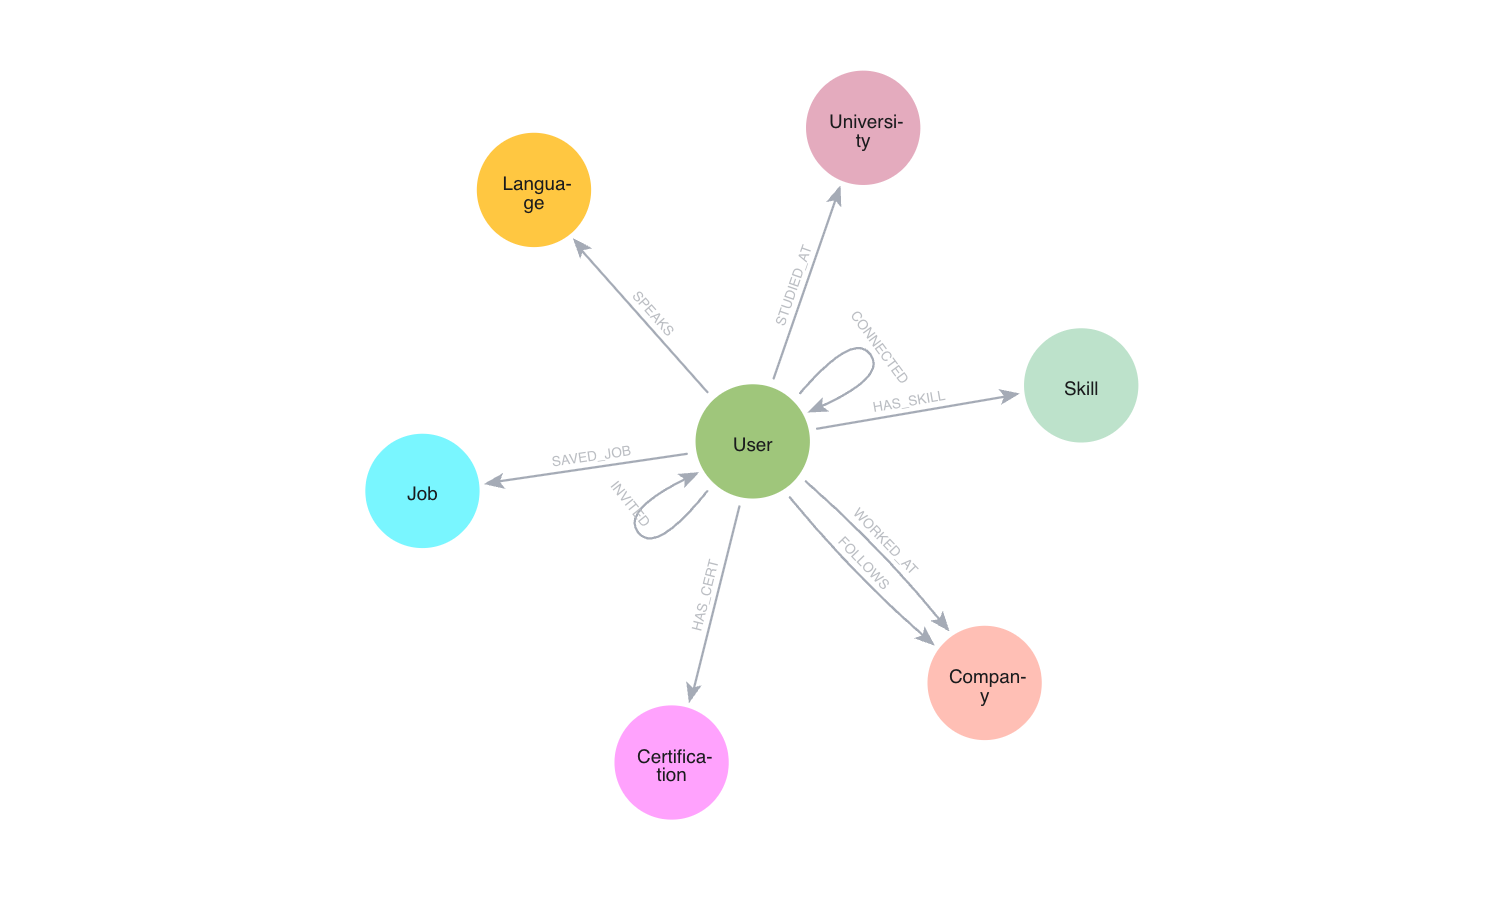
\includegraphics[width=0.9\textwidth]{images/schema.png}
	\caption{Estructura del grafo}
\end{figure}

\subsection*{Decisiones de modelado y motivaciones}

\begin{itemize}
	\item \textbf{Nombres normalizados:}
	      Se aplicó normalización a campos como \texttt{First \& Last Name} y \texttt{companyName} para evitar la creación de nodos duplicados en el grafo.
	      
	\item \textbf{Modelo centrado en el usuario:}
	      La estructura del grafo fue diseñada para tener al nodo \texttt{:User} como eje central, conectando a múltiples entidades relevantes del historial profesional y educativo. Esto permite analizar trayectorias, redes de colaboración y similitudes de forma eficiente.
	      
	\item \textbf{Relaciones con propiedades mínimas:}
	      Cada relación almacena únicamente la información necesaria (como fechas, cargo, nivel o dirección), buscando mantener el grafo lo más ligero posible sin perder contexto analítico.
	      
	\item \textbf{Separación de entidades conceptuales:}
	      Se optó por modelar entidades como \texttt{:Skill}, \texttt{:Certification} y \texttt{:Language} como nodos individuales en lugar de atributos simples, lo cual permite evaluar patrones agregados y buscar similitudes.
\end{itemize}

\subsection{Diagrama de arquitectura}
\begin{figure}[H]
	\centering
	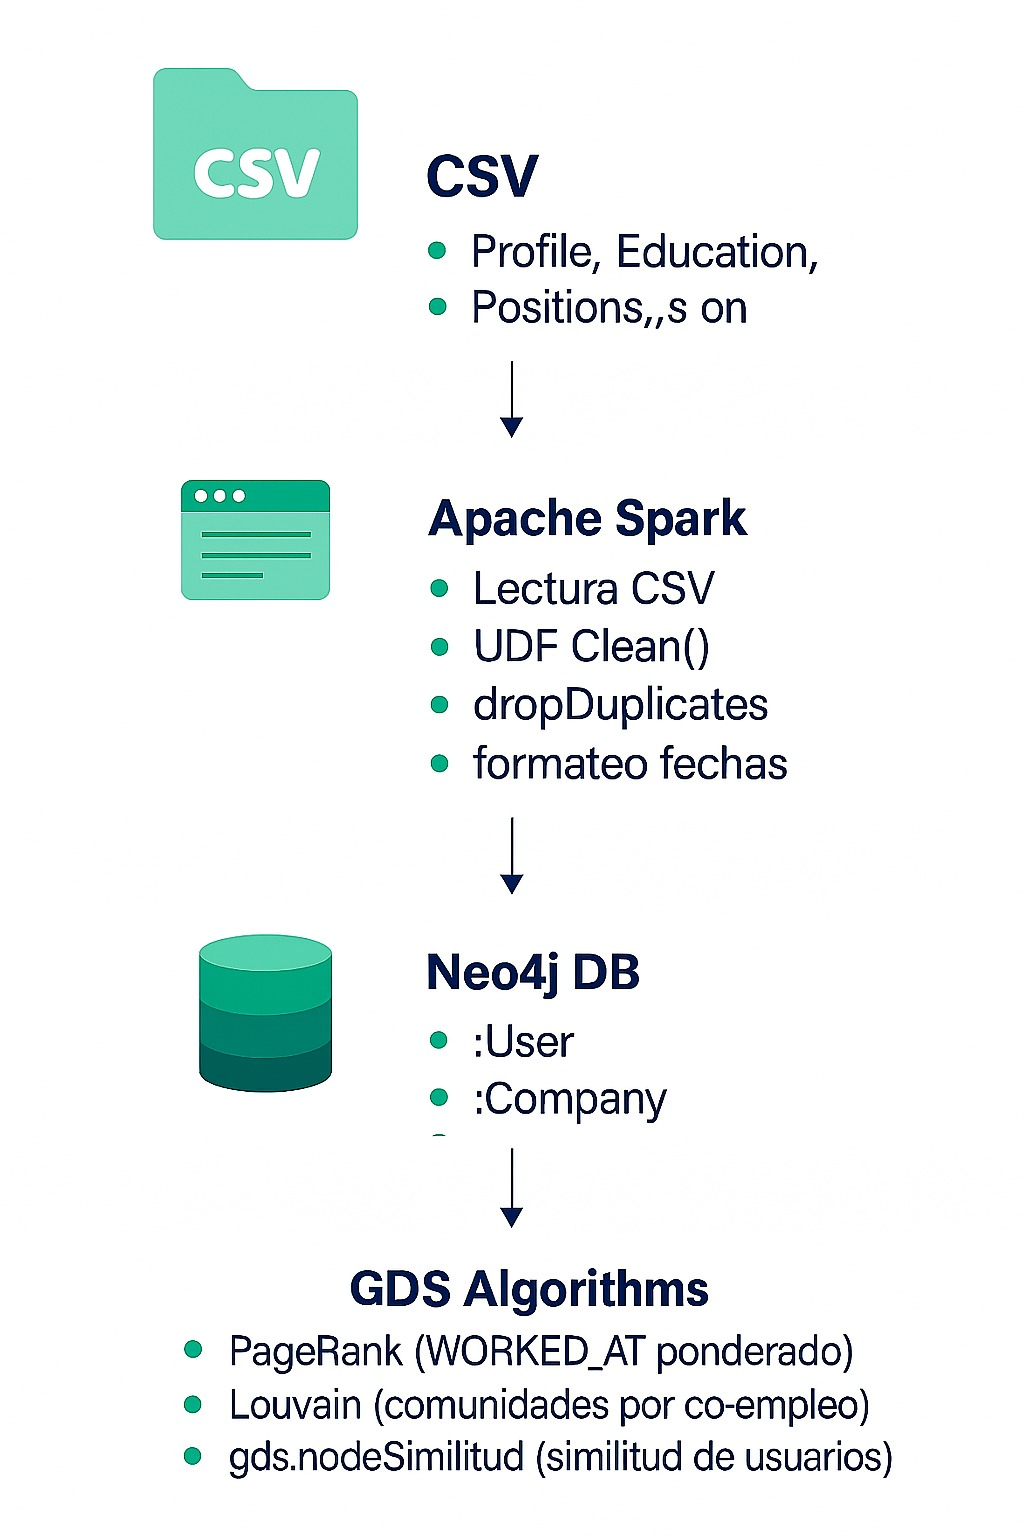
\includegraphics[width=0.5\textwidth]{images/arch-diag.jpeg}
	\caption{Diagrama de arquitectura del proceso}
\end{figure}
% CHECKTODO
%-----------------------------------------------
\section{Detección de comunidades y resultados}

En esta sección se presentan los tres algoritmos de análisis de grafos elegidos, cada uno representando una categoría: centralidad, detección de comunidades y similitud. A través de estos algoritmos, se analizaron patrones relevantes dentro del grafo.

\subsection{Algoritmo de Centralidad: \texttt{PageRank}}

\subsubsection*{Concepto del algoritmo}
PageRank es un algoritmo de centralidad que asigna una puntuación a los nodos basada en la importancia de sus conexiones. Originalmente fue diseñado para páginas web, pero en redes sociales profesionales permite identificar entidades (como empresas, en este caso) que concentran gran parte del flujo de vínculos laborales.

\subsubsection*{Aplicación en el grafo}
Se aplicó sobre un subgrafo que conecta usuarios con empresas mediante relaciones \texttt{WORKED\_AT}, ponderadas por la frecuencia del título laboral. Esto permite que cargos comunes como Engineer o Analyst influyan más en el peso de las conexiones, otorgando mayor importancia a empresas que atraen a perfiles similares.

\subsubsection*{Consulta Cypher}
\begin{center}
	\begin{lstlisting}
    CALL {
      CALL gds.pageRank.stream('pg', {
        relationshipWeightProperty: 'weight',
        dampingFactor: 0.85,
        maxIterations: 20,
        tolerance: 1e-6
      })
      YIELD nodeId, score
      RETURN nodeId, score
      ORDER BY score DESC
      LIMIT 10
    }
    
    MATCH (n)
    WHERE id(n) = nodeId
    OPTIONAL MATCH (n)-[r]->(m)
    RETURN 
      n AS nodo,
      r AS relacion,
      m AS nodoRelacionado,
      score
    ORDER BY score DESC
    \end{lstlisting}
\end{center}

\subsubsection*{Visualización}
\begin{figure}[H]
	\centering
	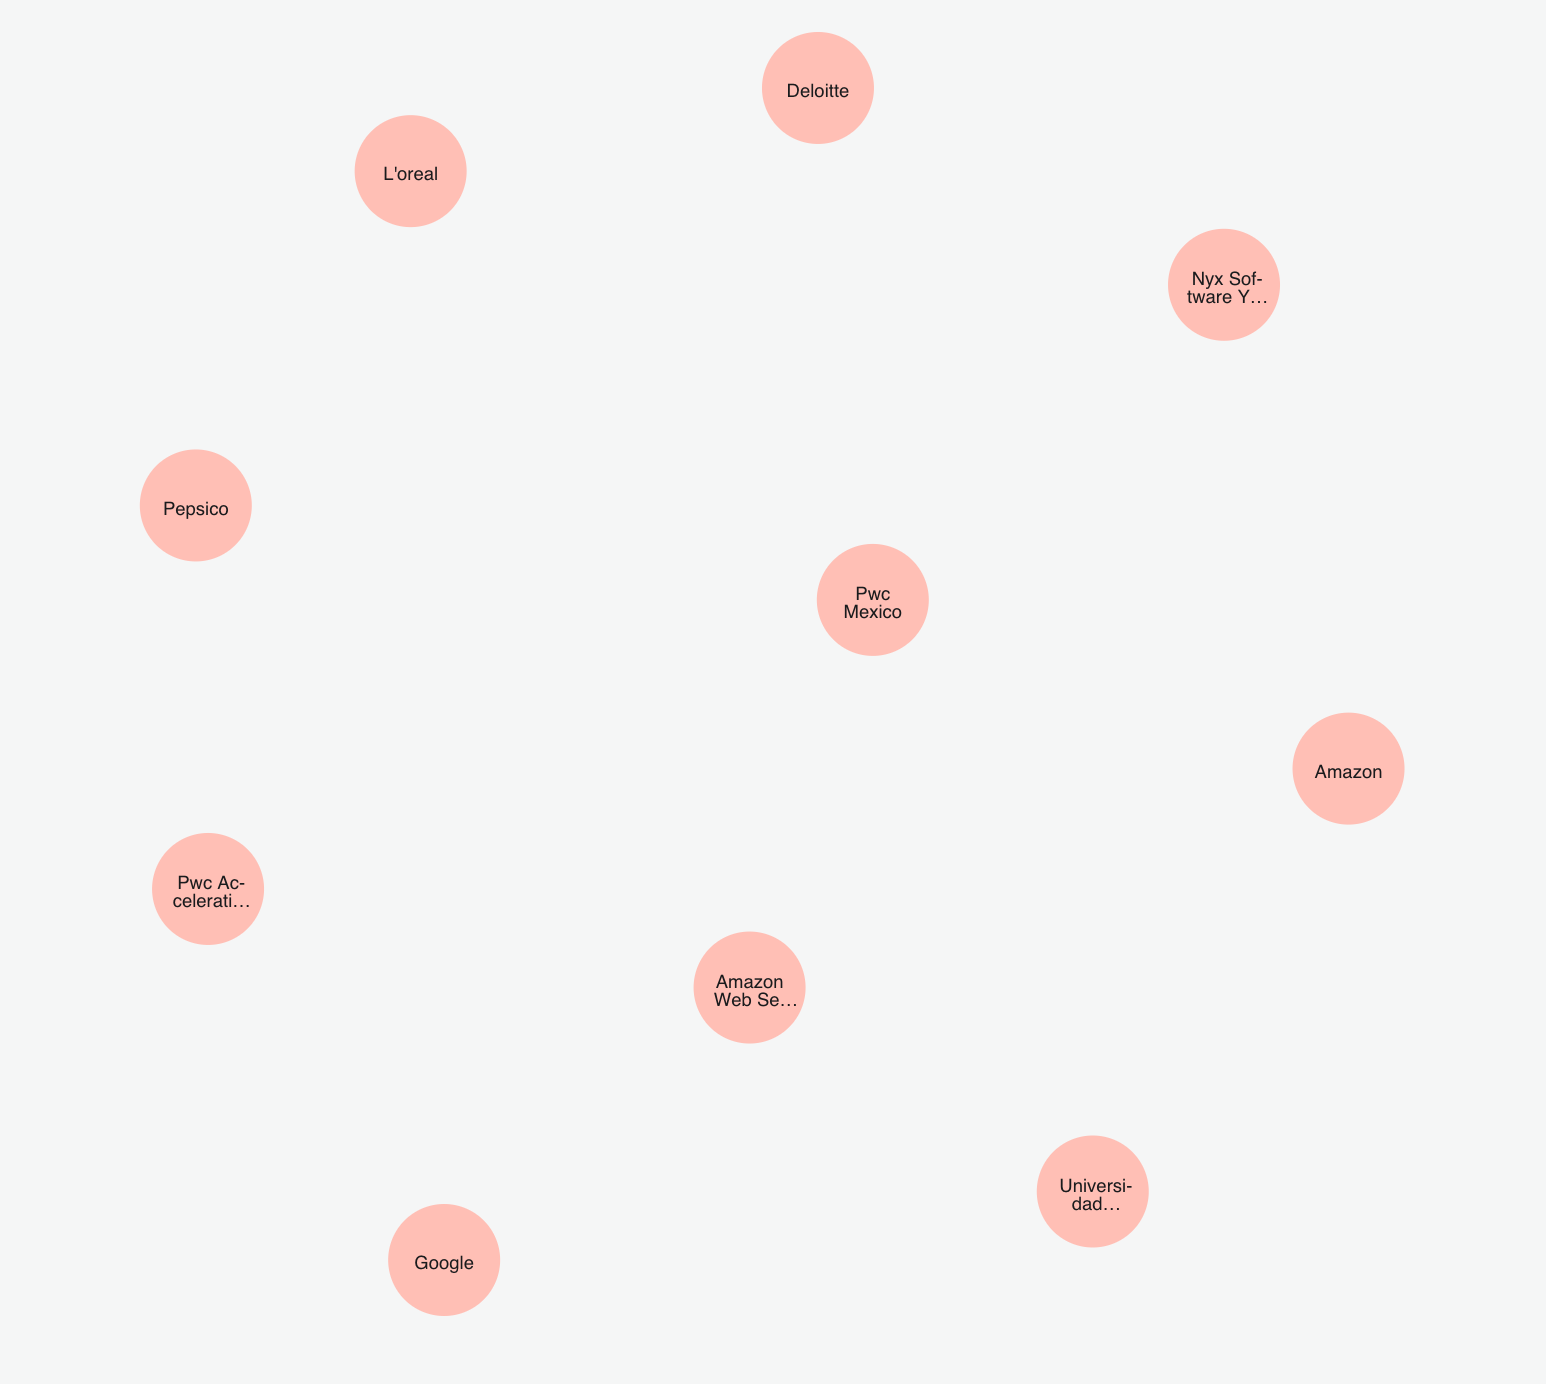
\includegraphics[width=0.68\textwidth]{images/pagerank.png}
	\caption{Nodos resultado del algoritmo PageRank}
\end{figure}

\subsubsection*{Resultados e interpretación}
\begin{table}[ht]
	\centering
	\begin{tabular}{|l|r|}
		\hline
		\textbf{Empresa}          & \textbf{PageRank} \\
		\hline
		Amazon Web Services       & 25.0125           \\
		Universidad Panamericana  & 11.7707           \\
		Amazon                    & 2.1900            \\
		Pwc Mexico                & 1.9350            \\
		L'oreal                   & 1.8075            \\
		Deloitte                  & 1.8075            \\
		Nyx Software Y Tecnologia & 1.8075            \\
		Pepsico                   & 1.5525            \\
		Pwc Acceleration Centers  & 1.5525            \\
		Google                    & 1.4250            \\
		\hline
	\end{tabular}
	\caption{Ranking de empresas según PageRank}
\end{table}

El análisis muestra un claro sesgo hacia Amazon Web Services (PageRank = 25), reflejo de que el entorno profesional del nodo más conectado gira principalmente en torno a AWS. La Universidad Panamericana (PageRank = 11,8) ocupa el segundo puesto, dado que los cuatro conjuntos de datos iniciales provienen de nosotros, estudiantes de esta institución y, por tanto, actúa como puente natural entre trayectorias. En la zona intermedia (PageRank 1,5–2,1) aparecen Amazon, PwC México, L’Oréal, Deloitte y Pepsico, nodos periféricos pero sólidos en nuestra red.

\subsection{Detección de comunidades: \texttt{Louvain}}

\subsubsection*{Concepto del algoritmo}
Louvain es un algoritmo de detección de comunidades que agrupa nodos densamente conectados optimizando una medida llamada modularidad. Es útil para encontrar clusters de usuarios que han trabajado en las mismas empresas o tienen trayectorias similares.

\subsubsection*{Aplicación en el grafo}
Se realizó una proyección usuario–usuario: dos usuarios se conectan si comparten al menos una empresa en común (a través de \texttt{WORKED\_AT}). Posteriormente, se ejecutó Louvain para agruparlos y se creó un nodo \texttt{Community} con relaciones explícitas hacia los usuarios (\texttt{BELONGS\_TO}) y hacia las empresas que los conectan (\texttt{HAS\_COMPANY}).

\subsubsection*{Consulta Cypher}
\begin{center}
	\begin{lstlisting}
    CALL gds.graph.project.cypher(
      'lc',
      'MATCH (u:User) RETURN id(u) AS id',
      '
        MATCH (u1:User)-[:WORKED_AT]->(c:Company)<-[:WORKED_AT]-(u2:User)
        WITH id(u1) AS source, id(u2) AS target, count(c) AS weight
        RETURN source, target, weight
      '
    );
    CALL gds.louvain.stream('lc', {
      relationshipWeightProperty: 'weight'
    })
    YIELD nodeId, communityId
    WITH gds.util.asNode(nodeId) AS usuario, communityId
    RETURN
      usuario.name    AS usuario,
      communityId     AS comunidad
    ORDER BY comunidad, usuario;
    CALL gds.louvain.write('lc', {
      writeProperty: 'communityId',
      relationshipWeightProperty: 'weight'
    })
    YIELD nodePropertiesWritten, communityCount;
    
    MATCH (u:User)
    WHERE u.communityId IS NOT NULL
    WITH collect(DISTINCT u.communityId) AS communities
    
    UNWIND communities AS commId
    
    CALL {
      WITH commId
      MATCH (u:User)
      WHERE u.communityId = commId
      RETURN count(u) AS numUsers
    }
    
    CALL {
      WITH commId
      MATCH (u:User)-[:WORKED_AT]->(c:Company)
      WHERE u.communityId = commId
      WITH c.name AS company, count(*) AS freq
      ORDER BY freq DESC
      RETURN collect(company)[0..5] AS top5Empresas
    }
    
    RETURN
      commId         AS Comunidad,
      numUsers       AS `# Usuarios`,
      top5Empresas   AS `Top-5 Empresas`
    ORDER BY `# Usuarios` DESC
    LIMIT 5;
    \end{lstlisting}
\end{center}

\subsubsection*{Visualización}
\begin{figure}[H]
	\centering
	
\includegraphics[width=1.1\textwidth]{images/communities.png}
	\caption{Comunidades resultantes del algoritmo de Louvain}
\end{figure}
\newpage
\subsubsection*{Resultados e interpretación}
\begin{table}[ht]
	\centering
	\begin{tabular}{|r|r|l|}
		\hline
		\textbf{Comunidad} & \textbf{\# Usuarios} & \textbf{Top-5 Empresas}                 \\
		\hline
		205                & 195                  & [Amazon Web Services]                   \\
		9                  & 98                   & [Universidad Panamericana, Klopp, Hal9] \\
		88                 & 16                   & [Amazon]                                \\
		306                & 14                   & [Nyx Software Y Tecnologia]             \\
		1341               & 14                   & [Pwc Mexico]                            \\
		\hline
	\end{tabular}
	\caption{Comunidades con sus usuarios y empresas destacadas}
\end{table}
El algoritmo Louvain identificó comunidades laborales con fuerte cohesión interna. La comunidad más grande está centrada en Amazon Web Services, con 195 usuarios, confirmando la amplia presencia en el grafo. La comunidad asociada a Universidad Panamericana, incluye 98 usuarios, lo cual es consistente con nuestra participación y la profesores en la red. Otras comunidades relevantes agrupan a empleados de empresas como Amazon, Nyx Software y Pwc.

\subsection{Similitud entre usuarios: \texttt{Según historial laboral compartido}}

\subsubsection*{Concepto del algoritmo}
El algoritmo \texttt{gds.nodeSimilarity} calcula la similitud estructural entre nodos del mismo tipo a partir de la superposición de sus vecinos. Utiliza métricas como la similitud de Jaccard, el coeficiente de solapamiento y la similitud coseno para determinar qué tan similares son dos nodos en función de sus conexiones en el grafo, y en este análisis se configuró con un umbral de 1.0, lo que significa que dos usuarios solo se consideran similares si han trabajado exactamente en las mismas empresas. A estos pares se les asignó una relación \texttt{SAME\_COMPANY} con una propiedad \texttt{score} que indica el nivel de similitud.

\subsubsection*{Aplicación en el grafo}
Se proyectó un grafo bipartito con nodos \texttt{User} y \texttt{Company}, conectados mediante \texttt{WORKED\_AT}, y se aplicó \texttt{nodeSimilarity} para identificar usuarios con trayectorias laborales idénticas. El resultado fue una red derivada de usuarios conectados por \texttt{SAME\_COMPANY}, que permitió analizar patrones de co-trabajo y calcular métricas como el grado promedio y la cantidad de pares de colegas por empresa.

\subsubsection*{Consulta Cypher}
\begin{center}
	\begin{lstlisting}
    CALL
      gds.graph.project(
        'userCompanyGraph',
        ['User', 'Company'],
        {WORKED_AT: {orientation: 'UNDIRECTED'}}
      );
    
    CALL
      gds.nodeSimilarity.write(
        'userCompanyGraph',
        {
          similarityCutoff: 1.0,
          writeRelationshipType: 'SAME_COMPANY',
          writeProperty: 'score'
        }
      )
      YIELD relationshipsWritten;
    
    MATCH ()-[r:SAME_COMPANY]->()
    RETURN count(r) AS pares_colegas;
    
    MATCH (u)-[:SAME_COMPANY]-()
    RETURN count(DISTINCT u) AS usuarios_con_colegas;
    
    MATCH ()-[r:SAME_COMPANY]-()
    RETURN 2.0 * count(r) / count(DISTINCT startNode(r)) AS grado_promedio;
    
    MATCH (c:Company)<-[:WORKED_AT]-(u:User)
    WITH c, count(u) AS empleados
    WHERE empleados > 1
    RETURN
      c.name AS empresa,
      empleados AS n_empleados,
      empleados * (empleados - 1) / 2 AS pares_colegas
    ORDER BY pares_colegas DESC
    LIMIT 10;
    
    \end{lstlisting}
\end{center}

\subsubsection*{Visualización}
\begin{figure}[H]
	\centering
	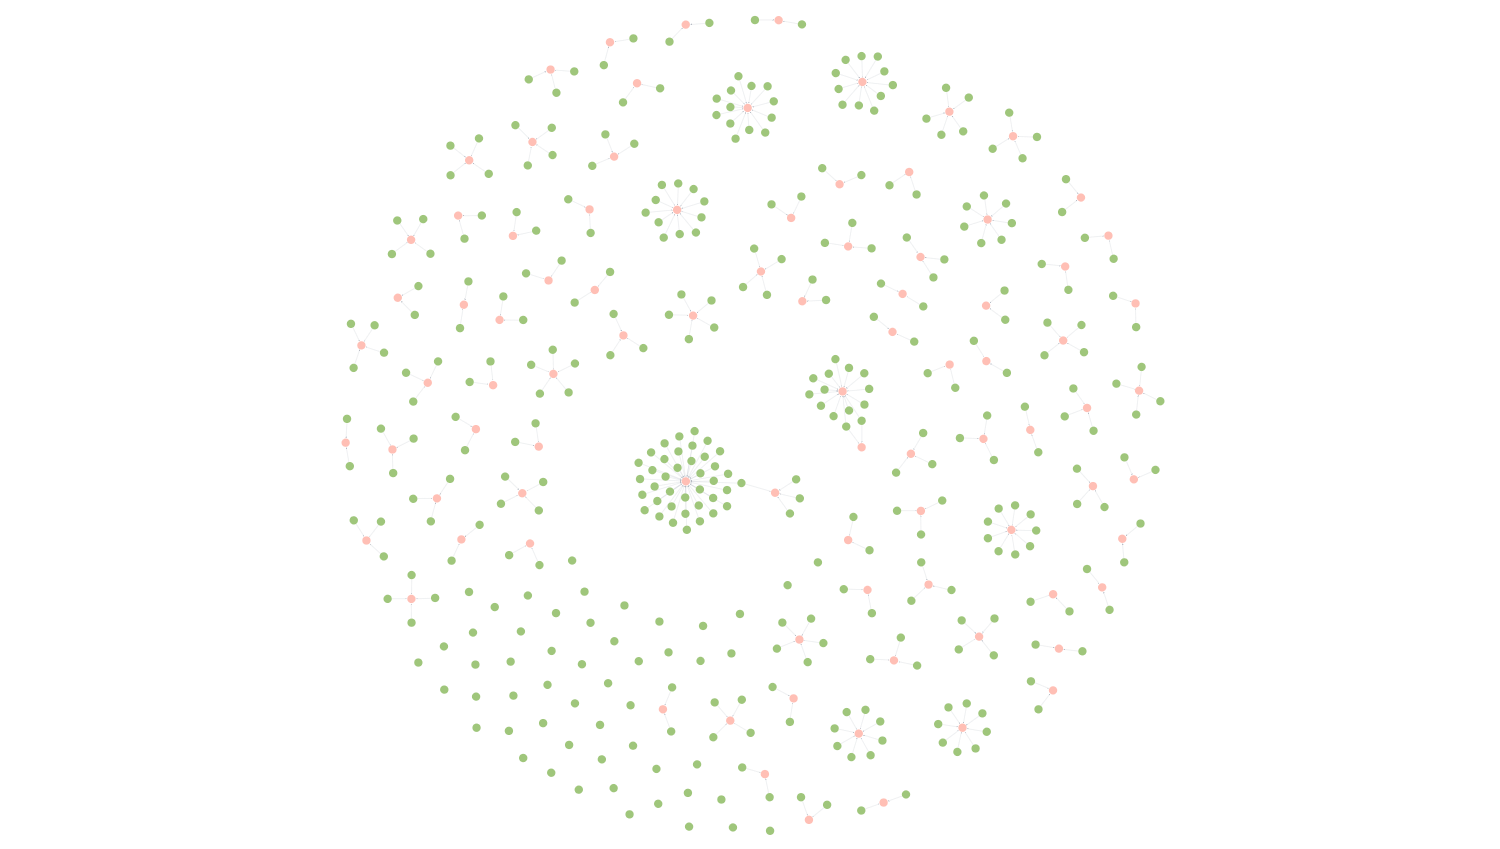
\includegraphics[width=1.1\textwidth]{images/similarity.png}
	\caption{Análisis de red de co-trabajo}
\end{figure}

\subsubsection*{Resultados e interpretación}
\begin{table}[H]
	\centering
	\begin{tabular}{|l|r|r|}
		\hline
		\textbf{Empresa}          & \textbf{N° Empleados} & \textbf{Pares de Colegas} \\
		\hline
		Amazon Web Services       & 195                   & 18,915                    \\
		Universidad Panamericana  & 92                    & 4,186                     \\
		Amazon                    & 16                    & 120                       \\
		Pwc Mexico                & 14                    & 91                        \\
		Nyx Software Y Tecnologia & 14                    & 91                        \\
		Deloitte                  & 13                    & 78                        \\
		L'oreal                   & 13                    & 78                        \\
		Pepsico                   & 11                    & 55                        \\
		Pwc Acceleration Centers  & 11                    & 55                        \\
		Google                    & 10                    & 45                        \\
		\hline
	\end{tabular}
	\caption{Empresas con mayor número de pares de colegas}
\end{table}
Como era de esperarse, Universidad Panamericana aparece entre las primeras, ya que nos incluye tanto a nosotros como a varios profesores conectados entre sí. Amazon Web Services destaca, aún más, con 18,915 pares de colegas, resultado directo de su alta cantidad de usuarios en el grafo, como hemos visto anteriormente. En ambos casos, la densidad de conexiones refleja múltiples trayectorias laborales compartidas y estructuras organizativas y académicas cohesionadas.

%-----------------------------------------------
\section{Conclusiones}

El análisis de la red profesional construida a partir de nuestros datos de LinkedIn revela varios puntos clave:

\begin{itemize}
	\item \textbf{Centralidad de empresas:} Amazon Web Services emerge como el nodo más influyente (PageRank $\approx$ 25), lo que indica que concentra el mayor flujo de conexiones laborales ponderadas por título.
	\item \textbf{Rol de la Universidad Panamericana:} Con un PageRank cercano a 12, la UP actúa como puente entre diferentes trayectorias, reflejo de que nuestros cuatro datasets iniciales provienen de esta institución.
	\item \textbf{Comunidades profesionales:} El algoritmo Louvain detectó subredes cohesionadas, especialmente alrededor de AWS y de la UP, así como clusters más pequeños en empresas como Nyx Software y PwC México.
	\item \textbf{Similitud de usuarios:} La métrica de “mismo empleador” (SAME\_COMPANY) confirma que AWS y la UP generan la mayoría de pares de colegas, evidenciando la densidad de sus estructuras internas.
\end{itemize}

Estos resultados nos dan una visión de dónde se concentra el talento de nuestra red y cómo fluye dentro de nuestra muestra, aunque quedan limitados al sesgo de datos de nosotros como estudiantes de la Universidad Panamericana.

\subsection{Implicaciones en el mundo real}
Identificar hubs como AWS y la UP nos ayuda a entender patrones de contratación y movilidad, y podría orientar estrategias de networking o de captación de talento. Sin embargo, al estar centrados en un grupo homogéneo, es necesario interpretar con cuidado la capacidad de generalizar estos hallazgos a poblaciones profesionales más amplias.

\subsection{Siguientes pasos}
\begin{itemize}
	\item \textbf{Ampliar cobertura de datos:} Incorporar información de otras fuentes mediante web scraping (ofertas de empleo, perfiles públicos, listados de empleados) para diversificar la muestra más allá de nuestros perfiles de LinkedIn.
	\item \textbf{Incluir nuevos tipos de relaciones:} Conseguir también conexiones de tipo \texttt{FOLLOWS}, \texttt{SKILL} o \texttt{CERT} de los demás usuarios con el objetivo de explorar afinidades basadas en intereses, habilidades o certificaciones.
	\item \textbf{Validación externa:} Confrontar nuestros resultados con métricas de mercado laboral (por ejemplo, volúmenes de contratación por sector) para calibrar la relevancia de los hubs identificados.
	\item \textbf{Mejorar el sesgo de la muestra:} Añadir perfiles de otros programas académicos o industrias, y evaluar cómo cambian las métricas de centralidad y comunidad al incorporar datos de usuarios con trayectorias distintas.
\end{itemize}
%-----------------------------------------------
\appendix

\section{Apéndice}

\subsection*{Link al repositorio}
https://github.com/enriquegomeztagle/MCD-DataMiningSocialNetworks-FinalProject-LinkedIn

\end{document}
